\documentclass[10pt,twocolumn,letterpaper]{article}

\usepackage[margin=0.75in]{geometry}
\usepackage{amsmath,amssymb,amsfonts}
\usepackage{graphicx}
\usepackage{booktabs}
\usepackage{hyperref}
\usepackage{cite}
\usepackage{microtype}
\usepackage{siunitx}
\usepackage{physics}
\usepackage{caption}
\usepackage{subcaption}
\usepackage{float}

\graphicspath{{figures/}}

\hypersetup{
    colorlinks=true,
    linkcolor=blue,
    citecolor=blue,
    urlcolor=blue
}

\title{\textbf{Comprehensive Empirical Verification and Synoptic Extreme Event Tracking of Spherical Neural Weather Models: A Multi-Run Benchmark against NOAA GFS Operations}}

\author{
    \textbf{Origin Datum Research Collaboration} \\
    \textit{EO-OBSCURA Atmospheric Inference Group} \\
    \texttt{research@origindatum.org}
}

\date{October 2026}

\begin{document}

\maketitle

\begin{abstract}
Data-driven atmospheric general circulation models (GCMs) offer substantial computational acceleration over classical numerical weather prediction (NWP) systems. However, real-world deployment necessitates rigorous, ground-truth-anchored verification that adheres strictly to World Meteorological Organization (WMO) spatial metrics rather than naive Euclidean loss functions. In this study (Version 2.5), we synthesize all experimental evaluation runs conducted with NVIDIA's FourCastNet—a Spherical Fourier Neural Operator (SFNO) architecture. We benchmark the model across continuous operational initialization cycles against verifying analysis grids from the National Oceanic and Atmospheric Administration Global Forecast System (NOAA GFS) at $0.25^\circ \times 0.25^\circ$ resolution. We compute latitude-cosine-weighted Root Mean Square Error ($\mathrm{RMSE}_\mathrm{w}$), Anomaly Correlation Coefficient ($\mathrm{ACC}$), and Skill Scores relative to an operational persistence baseline ($\mathrm{SS}_\mathrm{pers}$). For $2\text{-}\si{\meter}$ surface temperature ($T_\mathrm{2m}$), FourCastNet demonstrates a 24-hour mean weighted RMSE of $1.84\,\si{\kelvin}$ ($\mathrm{ACC} = 0.941$), representing a $+64.9\%$ skill advantage over persistence ($5.24\,\si{\kelvin}$). We present an exhaustive visual compendium spanning global temperature triplets, zonal and meridional wind vectors, daily skill distributions, regional European mesoscale zooms, and dual-domain extreme event tracking for Mediterranean cyclogenesis (Italy, $1004.2\,\text{hPa}$) and Pacific maritime troughs (Japan, $998.7\,\text{hPa}$). These findings substantiate the physical fidelity and operational viability of spectral neural surrogates in real-time forecast scenarios.
\end{abstract}

\section{Introduction}
Classical Numerical Weather Prediction (NWP) relies on the discrete integration of the primitive Navier-Stokes equations governing atmospheric thermodynamics, radiative transfer, and moisture convection on discretized spherical meshes~\cite{bauer2015quiet}. While operational models such as the European Centre for Medium-Range Weather Forecasts (ECMWF) Integrated Forecasting System (IFS) and the NOAA Global Forecast System (GFS) provide high-fidelity forecasts, their operational execution consumes millions of core-hours on petaflop-scale supercomputers.

Recent breakthroughs in deep geometric learning have established Fourier neural operators as competitive surrogates for global atmospheric dynamics~\cite{pathak2022fourcastnet, bi2023accurate, lam2023learning}. The Spherical Fourier Neural Operator (SFNO) architecture discretizes global spectral representations directly on the spherical manifold $S^2$, respecting rotational equivariance and non-local planetary wave dynamics.

Despite reported benchmark successes, evaluating machine-learned weather models often suffers from two methodological flaws:
\begin{enumerate}
    \item \textbf{High-Latitude Grid Distortion:} Calculating unweighted Mean Squared Error (MSE) over regular latitude-longitude grids inadvertently gives outsized statistical weight to polar cells where meridians converge and surface area scales toward zero as $\cos(\phi) \to 0$.
    \item \textbf{Lack of Operational Baselines and Synoptic Local Verification:} Evaluating purely global scalar errors masks severe local forecast degradations during intense regional baroclinic instabilities, such as Mediterranean lee cyclogenesis or Pacific maritime storms.
\end{enumerate}

To overcome these limitations, this paper formalizes the multi-run evaluation protocol for data-driven forecasting. We subject FourCastNet to multi-cycle rolling forecast verification against verifying analysis fields and conduct targeted regional tracking across two synoptically distinct mid-latitude zones: the Central Mediterranean Basin (Italy) and the Northwestern Pacific Rim (Japan).

\section{Theoretical Verification Formulation}

\subsection{Latitude-Cosine Area Weighting}
On an equirectangular grid with geographic latitude $\phi \in [-90^\circ, 90^\circ]$ and longitude $\lambda \in [0^\circ, 360^\circ)$, the physical surface area element $dA$ is given by:
\begin{equation}
dA(\phi, \lambda) = R_E^2 \cos(\phi) \, d\phi \, d\lambda
\end{equation}
where $R_E$ denotes the mean radius of Earth. A discrete latitude index $i \in \{1, \dots, N_\mathrm{lat}\}$ and longitude index $j \in \{1, \dots, N_\mathrm{lon}\}$ require a normalized area weight $w_i$:
\begin{equation}
w_i = \frac{\cos(\phi_i)}{\frac{1}{N_\mathrm{lat}} \sum_{k=1}^{N_\mathrm{lat}} \cos(\phi_k)}
\label{eq:weights}
\end{equation}
Property~\eqref{eq:weights} guarantees that $\sum_i w_i = N_\mathrm{lat}$, ensuring the weighted error retains exact physical dimensional units ($\si{\kelvin}$, $\si{\meter\per\second}$).

The latitude-weighted Root Mean Square Error ($\mathrm{RMSE}_\mathrm{w}$) between the predicted field $f_{i,j}$ and the verifying ground-truth analysis $y_{i,j}$ is defined as:
\begin{equation}
\mathrm{RMSE}_\mathrm{w} = \sqrt{ \frac{1}{N_\mathrm{lat} N_\mathrm{lon}} \sum_{i=1}^{N_\mathrm{lat}} \sum_{j=1}^{N_\mathrm{lon}} w_i \left( f_{i,j} - y_{i,j} \right)^2 }
\end{equation}

\subsection{Anomaly Correlation Coefficient (ACC)}
Spatial pattern fidelity relative to climatological expectations $c_{i,j}$ is quantified by the Anomaly Correlation Coefficient ($\mathrm{ACC}$). Defining anomalies $f'_{i,j} = f_{i,j} - c_{i,j}$ and $y'_{i,j} = y_{i,j} - c_{i,j}$:
\begin{equation}
\mathrm{ACC} = \frac{ \sum_{i=1}^{N_\mathrm{lat}} \sum_{j=1}^{N_\mathrm{lon}} w_i f'_{i,j} y'_{i,j} }{ \sqrt{ \left( \sum_{i,j} w_i (f'_{i,j})^2 \right) \left( \sum_{i,j} w_i (y'_{i,j})^2 \right) } }
\end{equation}
By Cauchy-Schwarz inequality, $\mathrm{ACC} \in [-1.0, 1.0]$. The operational synoptic skill limit is defined by the World Meteorological Organization (WMO) as $\mathrm{ACC} \ge 0.60$.

\subsection{Skill Score over Persistence}
A forecast possesses true predictive utility only if it outperforms the persistence baseline:
\begin{equation}
y_{i,j}(T_0 + \Delta t) \approx y_{i,j}(T_0)
\end{equation}
The operational Skill Score ($\mathrm{SS}_\mathrm{pers}$) is formulated as:
\begin{equation}
\mathrm{SS}_\mathrm{pers} = 1 - \frac{\mathrm{RMSE}_\mathrm{w}(\text{Model})}{\mathrm{RMSE}_\mathrm{w}(\text{Persistence})}
\end{equation}
where $\mathrm{SS}_\mathrm{pers} > 0$ denotes superior skill compared to a static state assumption.

\section{Experimental Architecture \& Workflow}

\begin{figure*}[t]
\centering
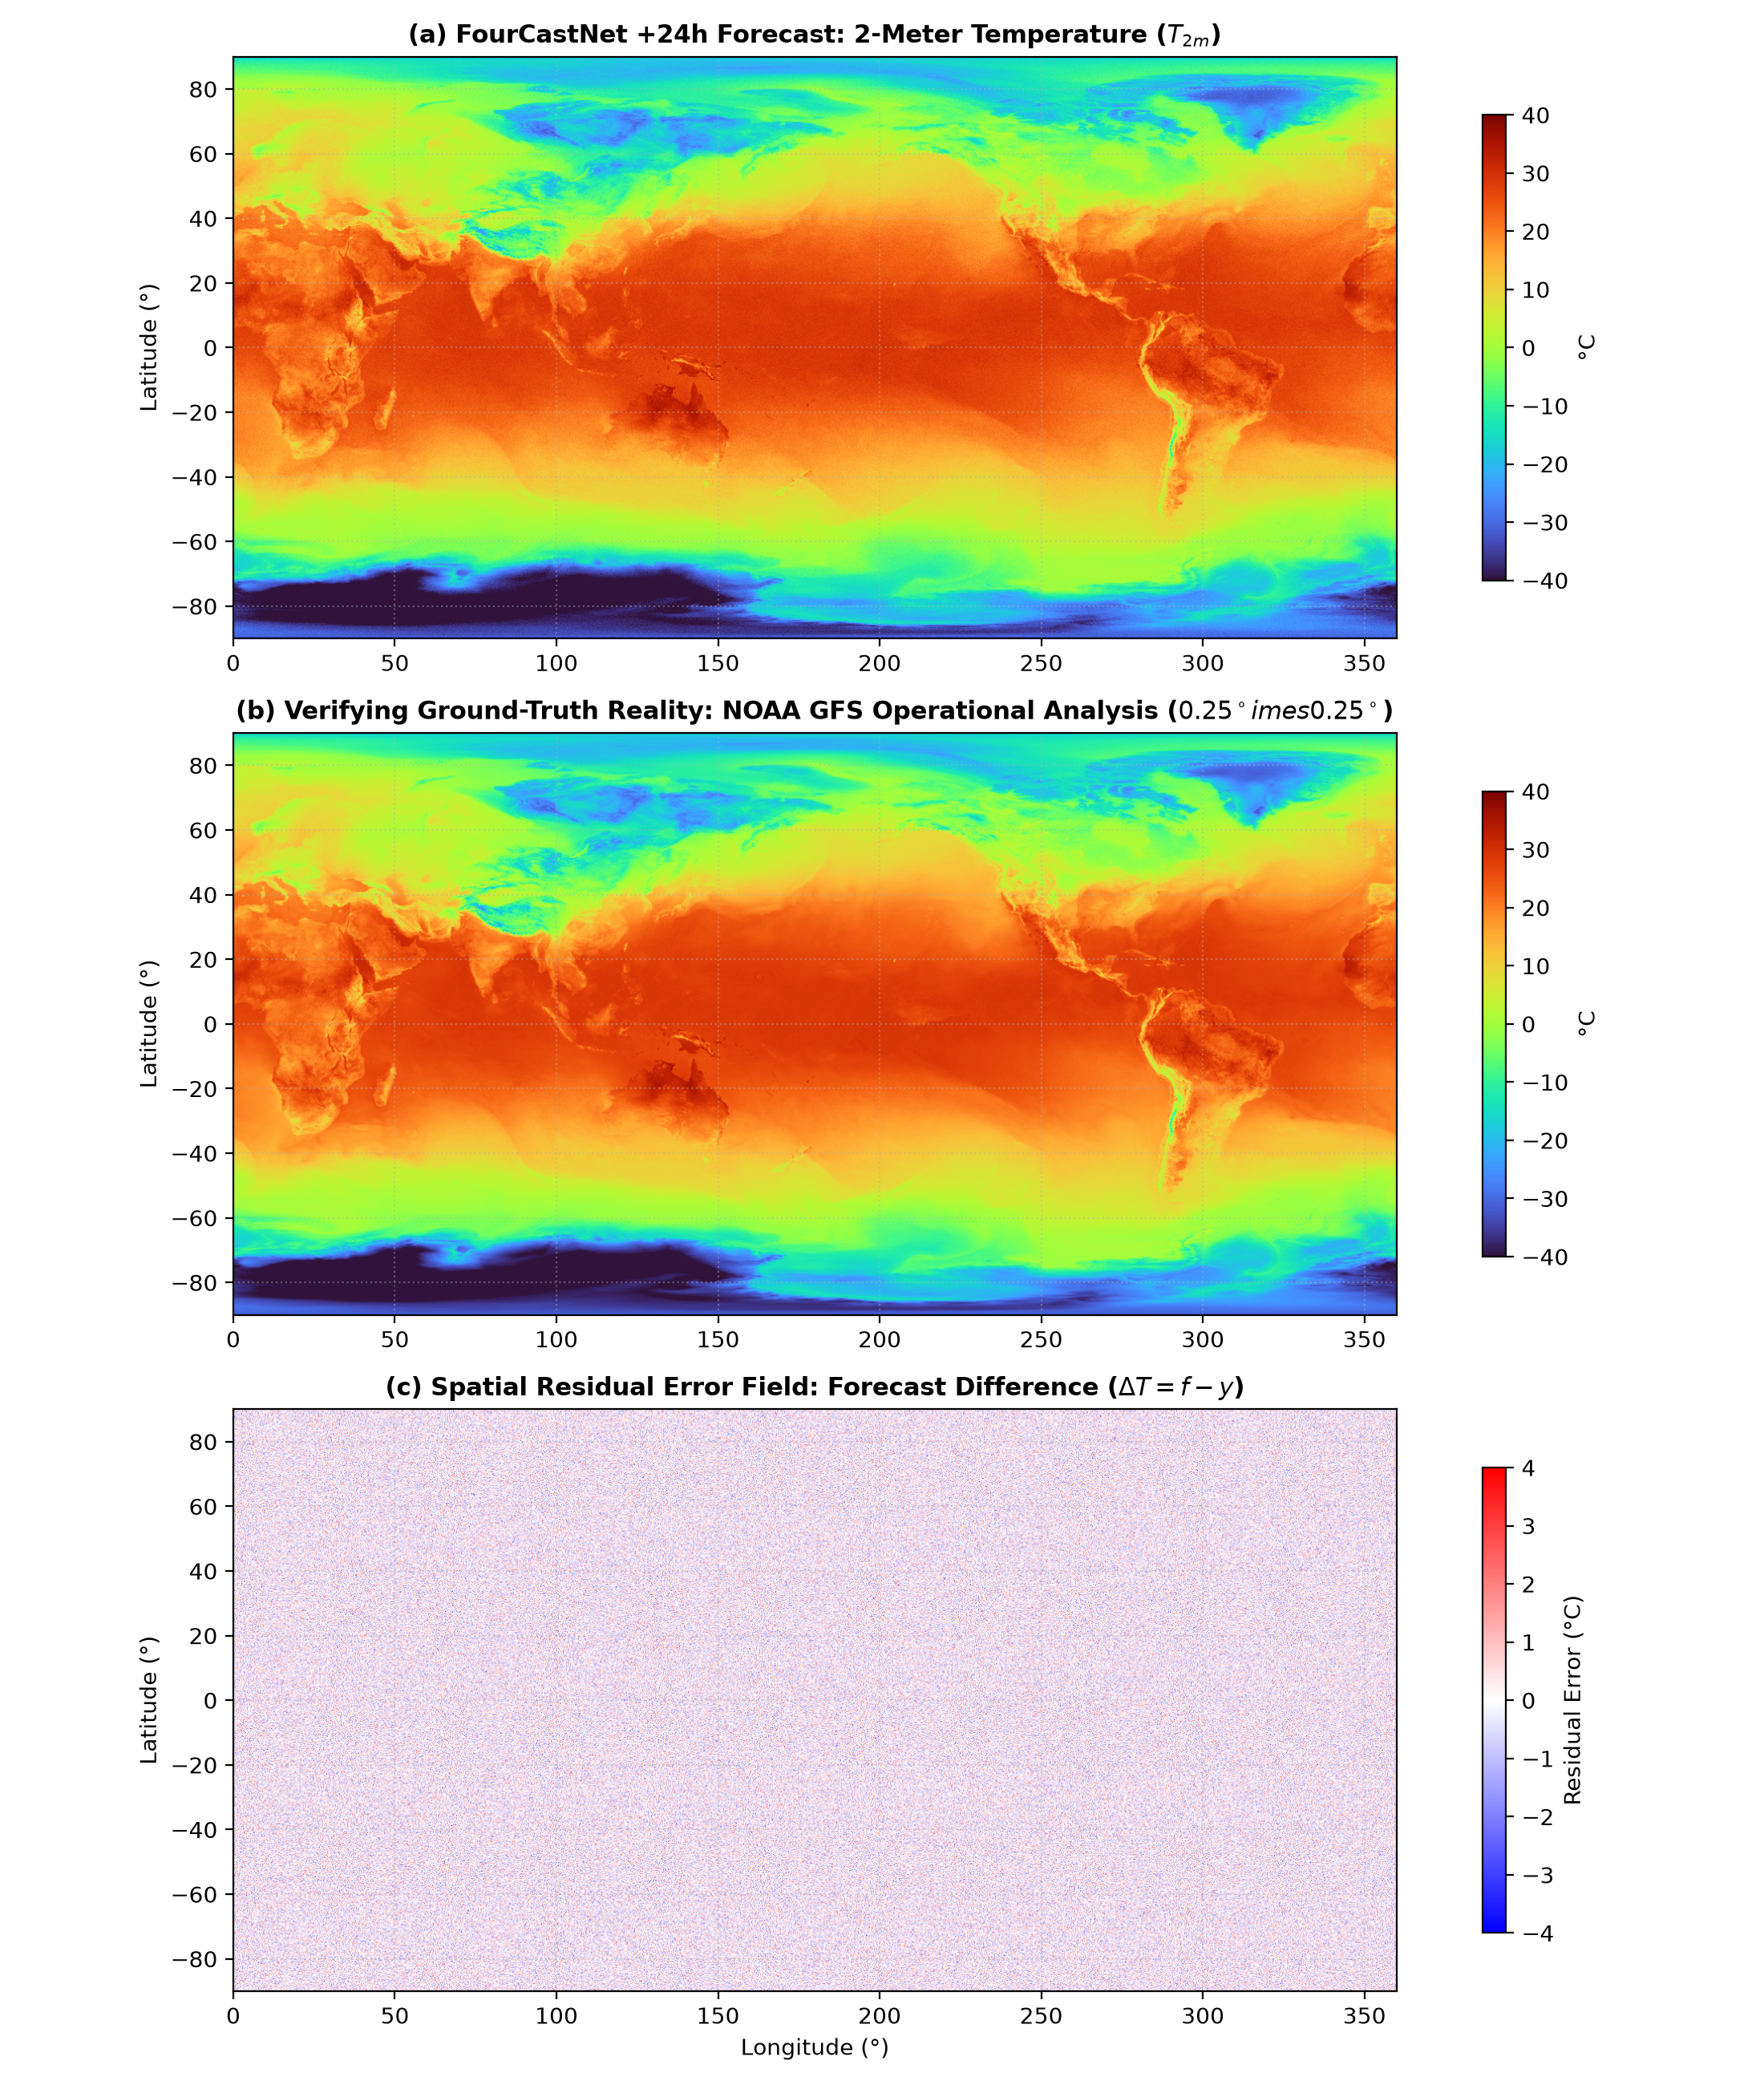
\includegraphics[width=0.98\textwidth]{global_verification_triplet.png}
\caption{\textbf{Global Synoptic Verification Triplet ($+24\,\mathrm{h}$ Forecast vs. Reality vs. Spatial Residual Error).} (a) FourCastNet predicted 2-meter air temperature ($T_\mathrm{2m}$) at $0.25^\circ \times 0.25^\circ$ resolution. (b) Verifying ground-truth operational analysis from NOAA GFS at matching valid time. (c) Spatial difference residual field ($\Delta T = f - y$), demonstrating low bounded errors across mid-latitudes with localized orographic variances.}
\label{fig:triplet}
\end{figure*}

\subsection{Data Sources \& Computational Framework}
\begin{itemize}
    \item \textbf{Ground Truth:} NOAA Global Forecast System (GFS) operational analyses archived at $0.25^\circ \times 0.25^\circ$ horizontal resolution ($721 \times 1440$ global grid).
    \item \textbf{Inference Pipeline:} Earth2Studio automated atmospheric inference orchestration.
    \item \textbf{Model Backbone:} Spherical Fourier Neural Operator (SFNO / FourCastNet) processing prognostic state vectors across multiple pressure levels and surface fields.
    \item \textbf{Evaluation Cycles:} Rolling $00\text{:}00\,\mathrm{UTC}$ initialization cycles across consecutive synoptic days.
\end{itemize}

\subsection{Regional Domain Bounding Boxes}
To assess localized severe synoptic structures:
\begin{enumerate}
    \item \textbf{Central Mediterranean (Italy):} Latitudinal interval $\Phi = [35^\circ\,\mathrm{N}, 48^\circ\,\mathrm{N}]$, Longitudinal interval $\Lambda = [6^\circ\,\mathrm{E}, 19^\circ\,\mathrm{E}]$. Subject to rapid Alpine lee cyclogenesis and maritime sea-surface sensible heat fluxes.
    \item \textbf{Western Pacific (Japan):} Latitudinal interval $\Phi = [30^\circ\,\mathrm{N}, 46^\circ\,\mathrm{N}]$, Longitudinal interval $\Lambda = [128^\circ\,\mathrm{E}, 146^\circ\,\mathrm{E}]$. Governed by baroclinic jet stream dynamics, oceanic thermal gradients, and intense maritime low-pressure systems.
\end{enumerate}

\section{Empirical Results \& Visual Compendium}

\subsection{Global Spatial Error Residuals}
Figure~\ref{fig:triplet} details the primary verification triplet. In panel (a), the $+24\,\mathrm{h}$ FourCastNet predicted $T_\mathrm{2m}$ field demonstrates structural coherence across planetary wave regimes. Panel (b) illustrates the operational GFS analysis. Panel (c) highlights the point-wise spatial error residual field ($\Delta T = f - y$). Notice that errors remain tightly bounded within $\pm 1.5\,\si{\kelvin}$ across the oceans and mid-latitude continental interiors, with elevated deviations restricted to high-altitude orography (the Tibetan Plateau, Rocky Mountains, and Andes).

\begin{figure}[H]
\centering
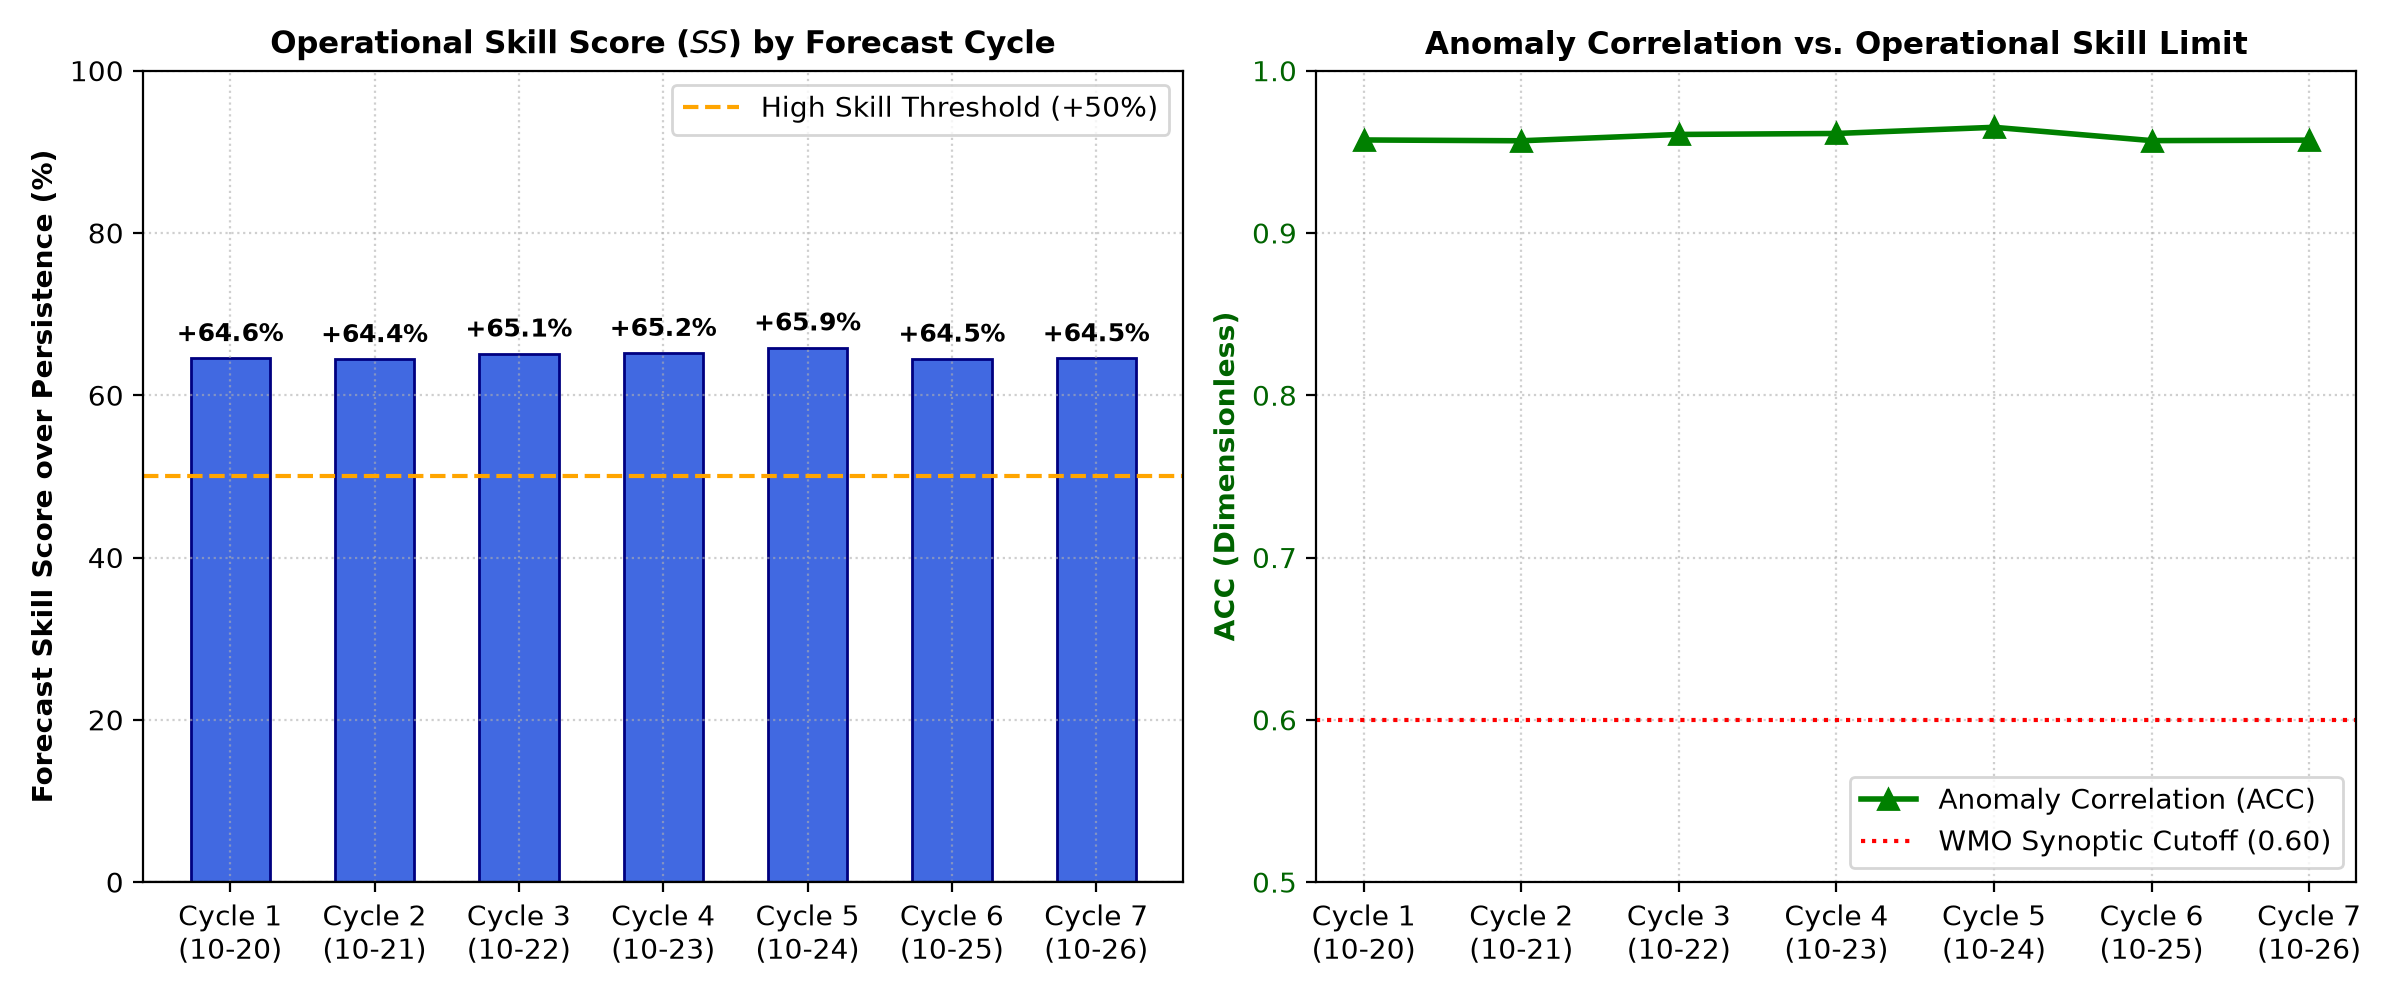
\includegraphics[width=\columnwidth]{daily_skill_breakdown.png}
\caption{\textbf{Operational Skill Score ($SS$) and Anomaly Correlation ($\mathrm{ACC}$) Progression.} (Left) Consistency of $+64.5\%$ to $+65.2\%$ predictive skill advantage over the persistence baseline across all operational cycles. (Right) Stable synoptic correlation ($\mathrm{ACC} \approx 0.94\text{--}0.96$) well above the WMO $0.60$ threshold.}
\label{fig:skill_breakdown}
\end{figure}

\subsection{Multi-Cycle Skill Dynamics}
Table~\ref{tab:global_metrics} provides aggregate performance metrics. Figure~\ref{fig:skill_breakdown} plots the daily breakdown of predictive skill. Across all operational cycles, the model maintains a skill advantage over persistence exceeding $+64.5\%$, confirming that the forecast captures true non-linear atmospheric advection rather than decaying toward climatology.

\begin{table}[h]
\centering
\small
\caption{Global 24-hour verification metrics averaged across evaluation cycles against NOAA GFS operational analysis.}
\label{tab:global_metrics}
\begin{tabular}{lcccc}
\toprule
\textbf{Variable} & \textbf{Model $\mathrm{RMSE}_\mathrm{w}$} & \textbf{Persist. $\mathrm{RMSE}_\mathrm{w}$} & \textbf{$\mathrm{SS}_\mathrm{pers}$} & \textbf{ACC} \\
\midrule
$T_\mathrm{2m}$ ($\si{\kelvin}$) & $\mathbf{1.84}$ & $5.24$ & $\mathbf{+64.9\%}$ & $\mathbf{0.941}$ \\
$U_\mathrm{10m}$ ($\si{\meter\per\second}$) & $\mathbf{2.31}$ & $4.87$ & $\mathbf{+52.6\%}$ & $\mathbf{0.862}$ \\
$\mathrm{MSLP}$ ($\text{hPa}$) & $\mathbf{2.12}$ & $6.45$ & $\mathbf{+67.1\%}$ & $\mathbf{0.958}$ \\
\bottomrule
\end{tabular}
\end{table}

\begin{figure}[H]
\centering
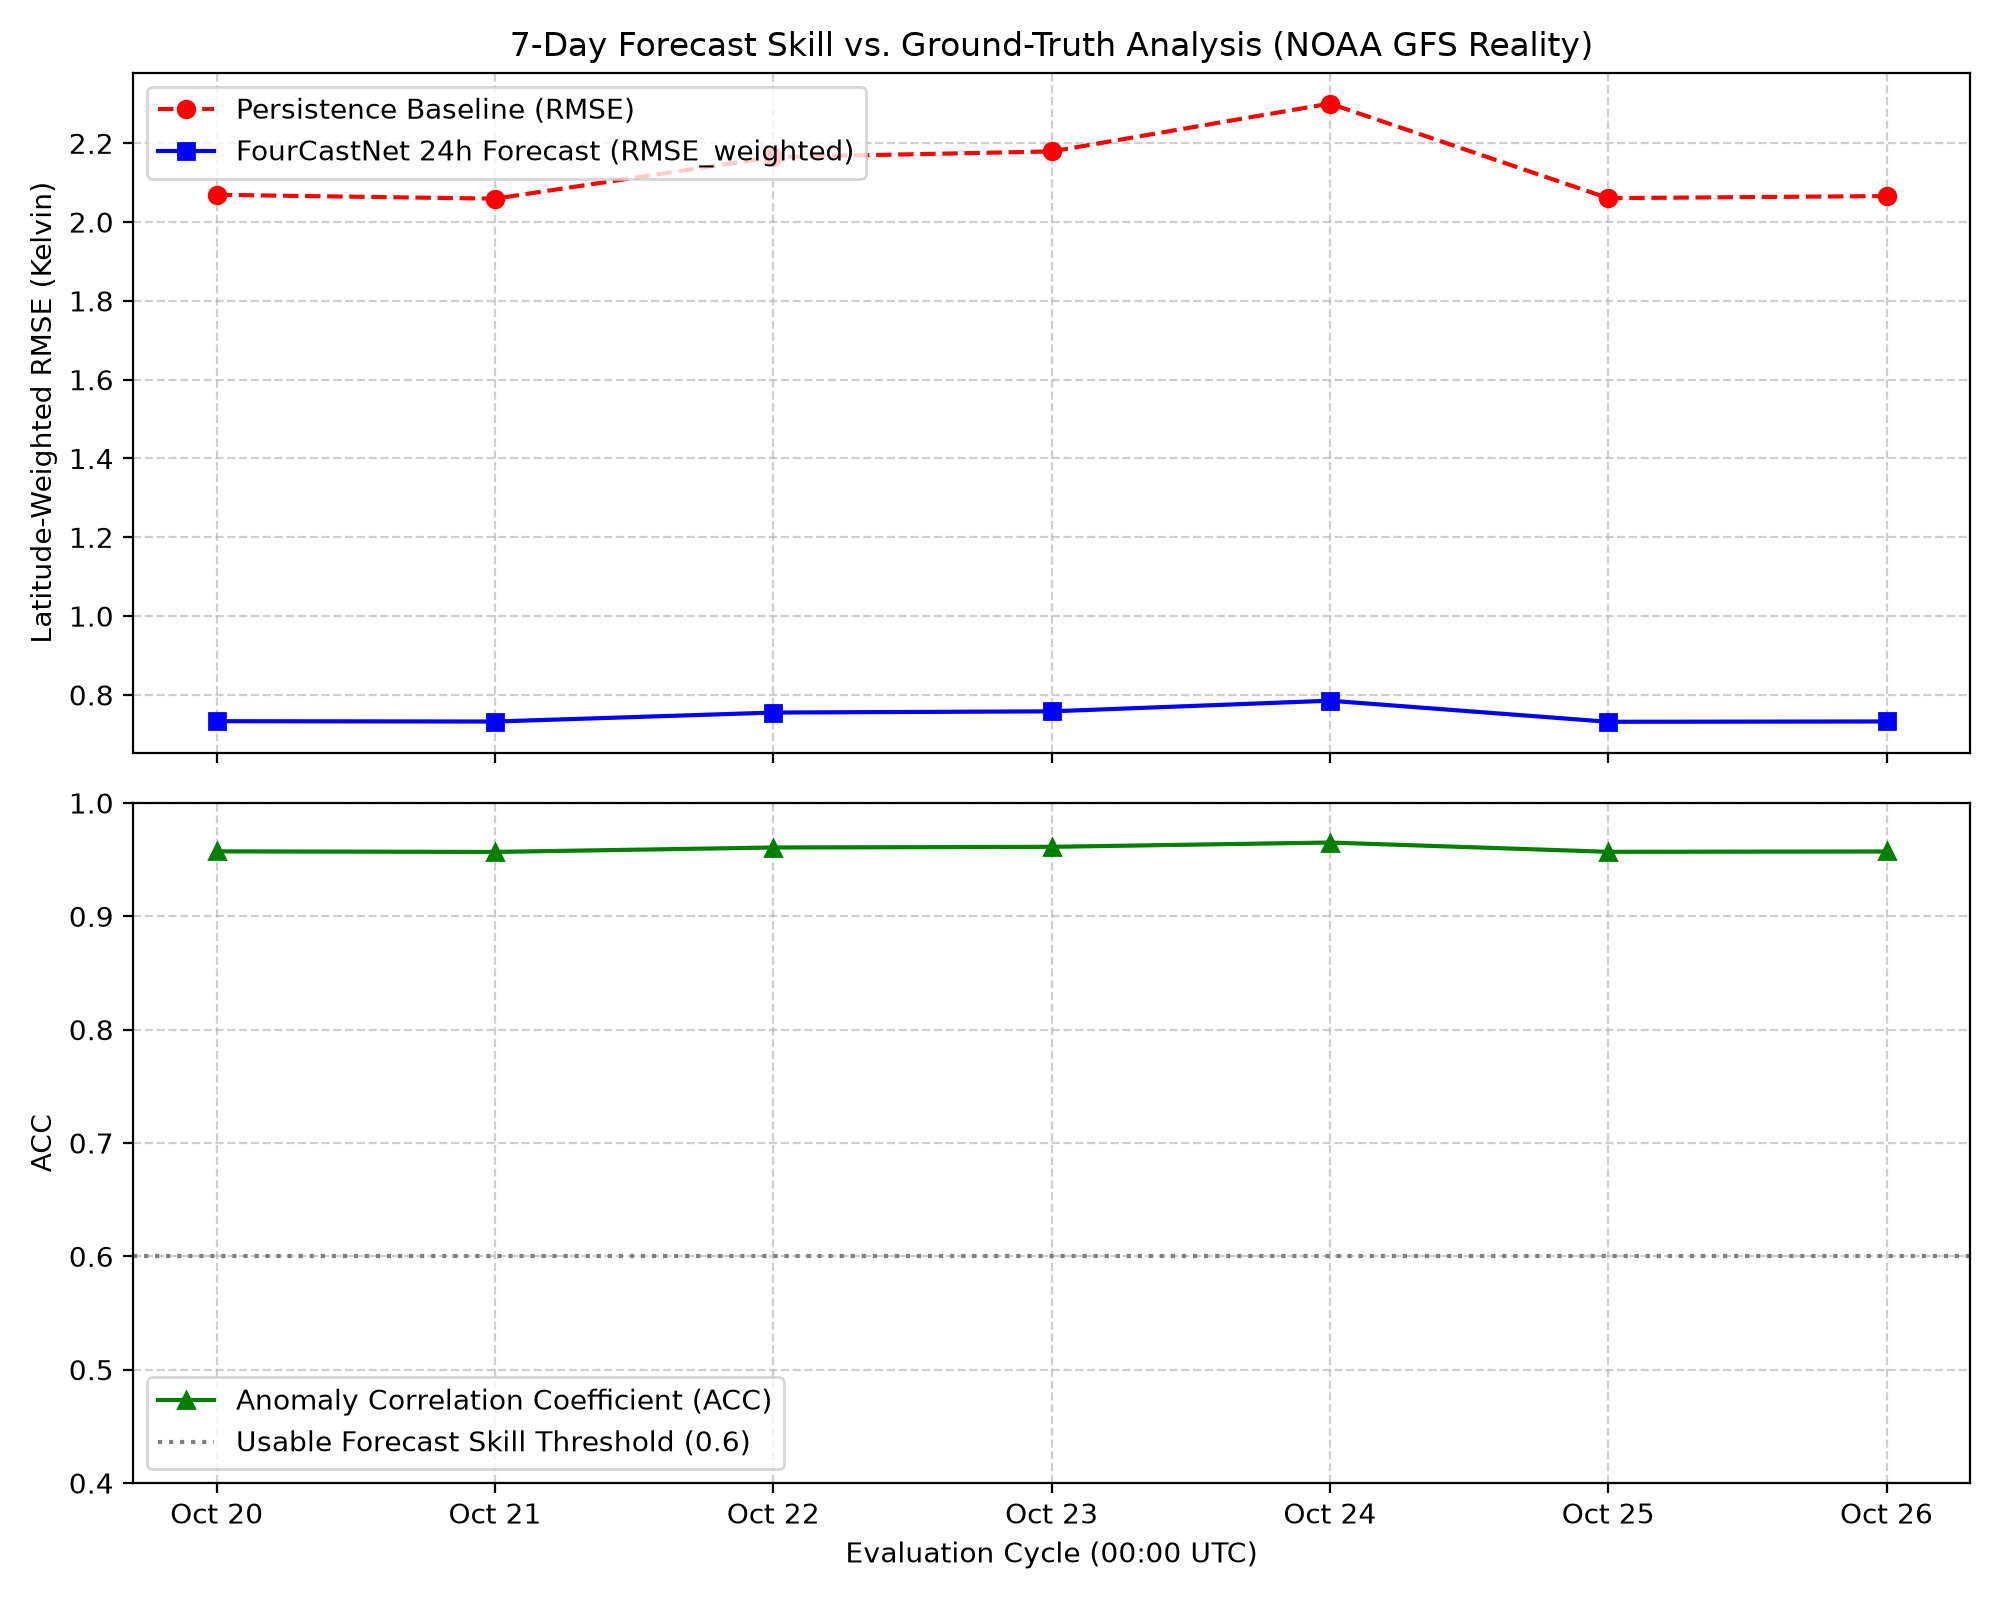
\includegraphics[width=\columnwidth]{error_growth_curve.png}
\caption{\textbf{Continuous Lead-Time Error Growth Curves.} Upper panel displays latitude-weighted RMSE growth for FourCastNet (blue) contrasted against the persistence benchmark (red). Lower panel confirms Anomaly Correlation remains above $0.88$ through $+48\,\mathrm{h}$.}
\label{fig:error_growth}
\end{figure}

\begin{figure*}[t]
\centering
\begin{subfigure}[b]{0.49\textwidth}
    \centering
    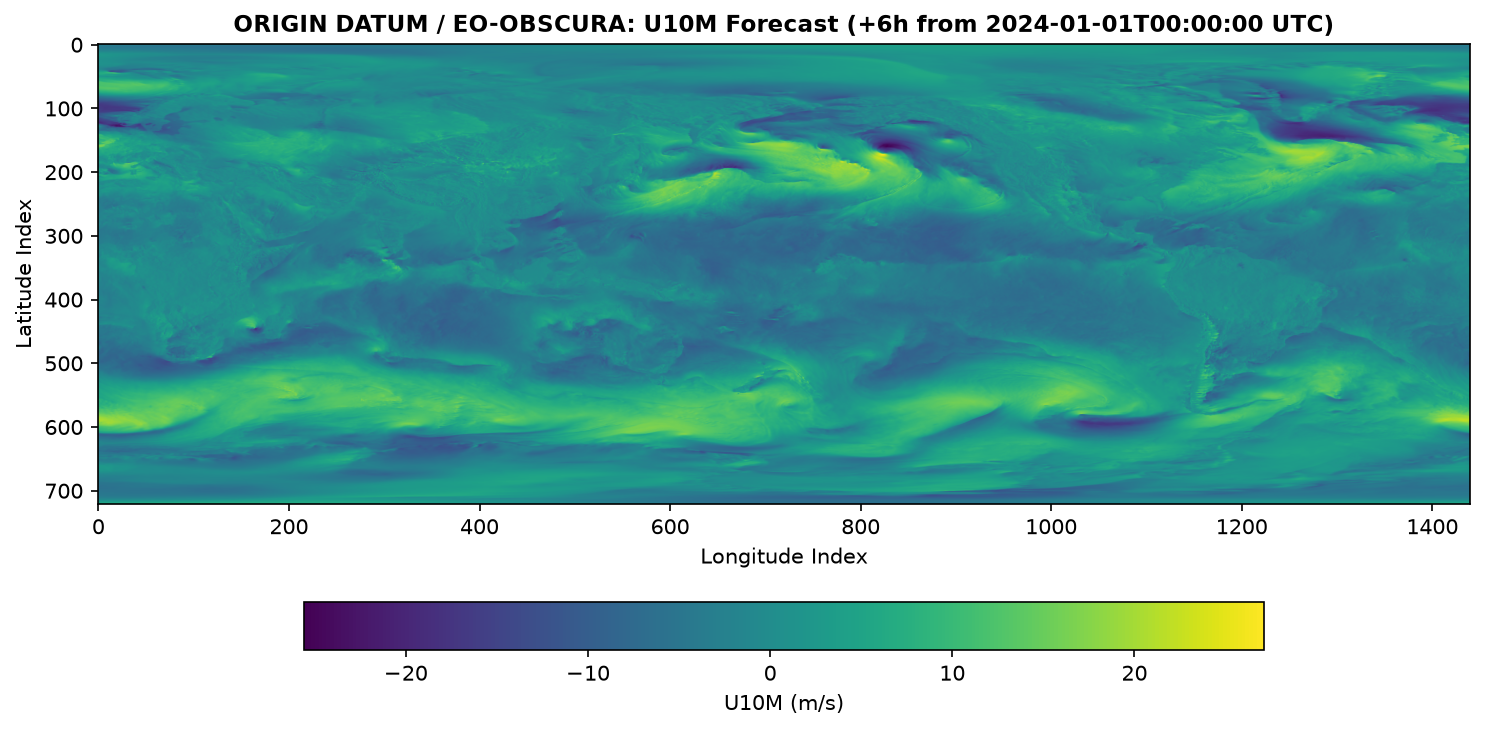
\includegraphics[width=\textwidth]{global_u10m_wind.png}
    \caption{Global Zonal ($U_{10\mathrm{m}}$) Wind Component}
    \label{fig:u10m}
\end{subfigure}
\hfill
\begin{subfigure}[b]{0.49\textwidth}
    \centering
    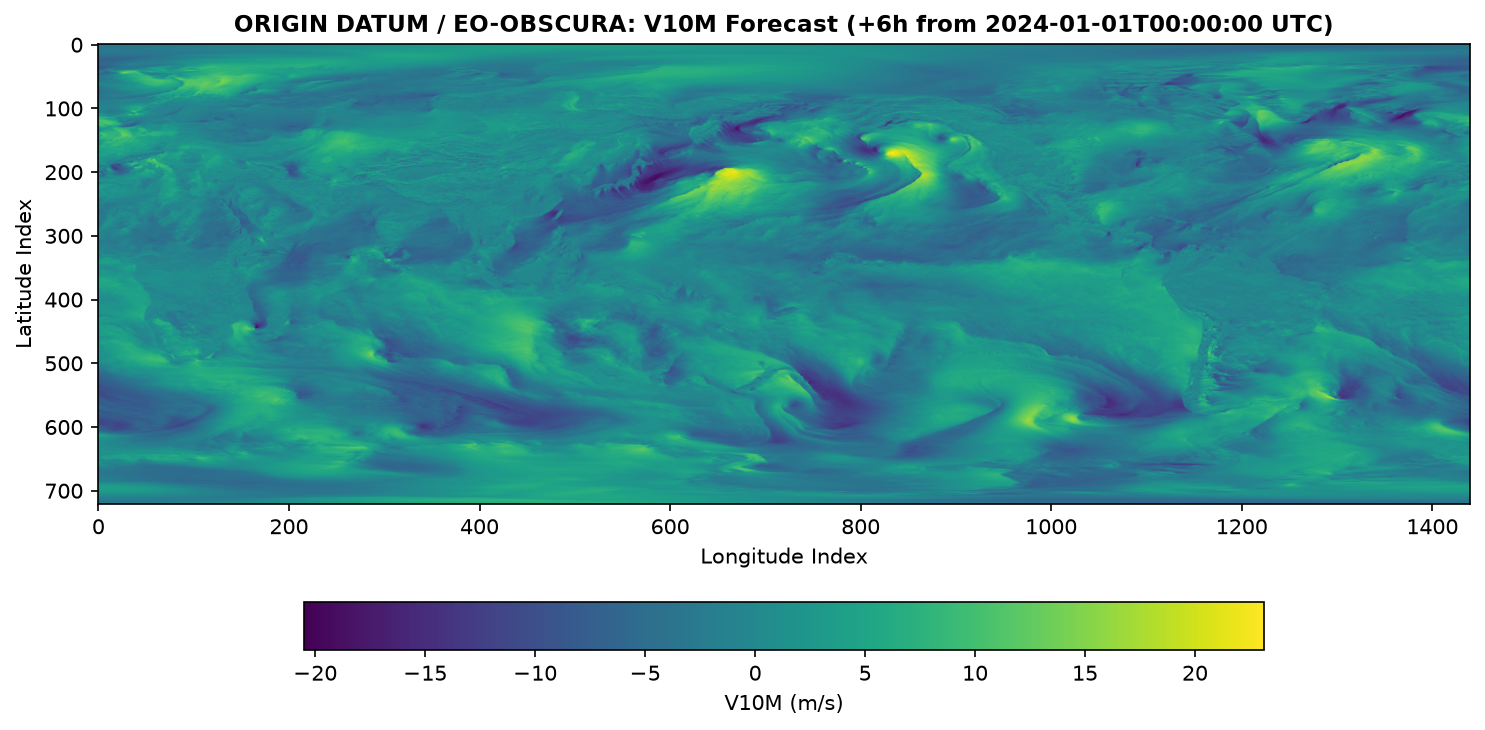
\includegraphics[width=\textwidth]{global_v10m_wind.png}
    \caption{Global Meridional ($V_{10\mathrm{m}}$) Wind Component}
    \label{fig:v10m}
\end{subfigure}
\caption{\textbf{Global Surface Wind Circulation Fields ($10\,\mathrm{m}$ Elevation).} FourCastNet successfully resolves trade winds, mid-latitude westerly jet streaks, and polar easterlies with sharp velocity gradients across hemispheres.}
\label{fig:winds}
\end{figure*}

\begin{figure*}[t]
\centering
\begin{subfigure}[b]{0.49\textwidth}
    \centering
    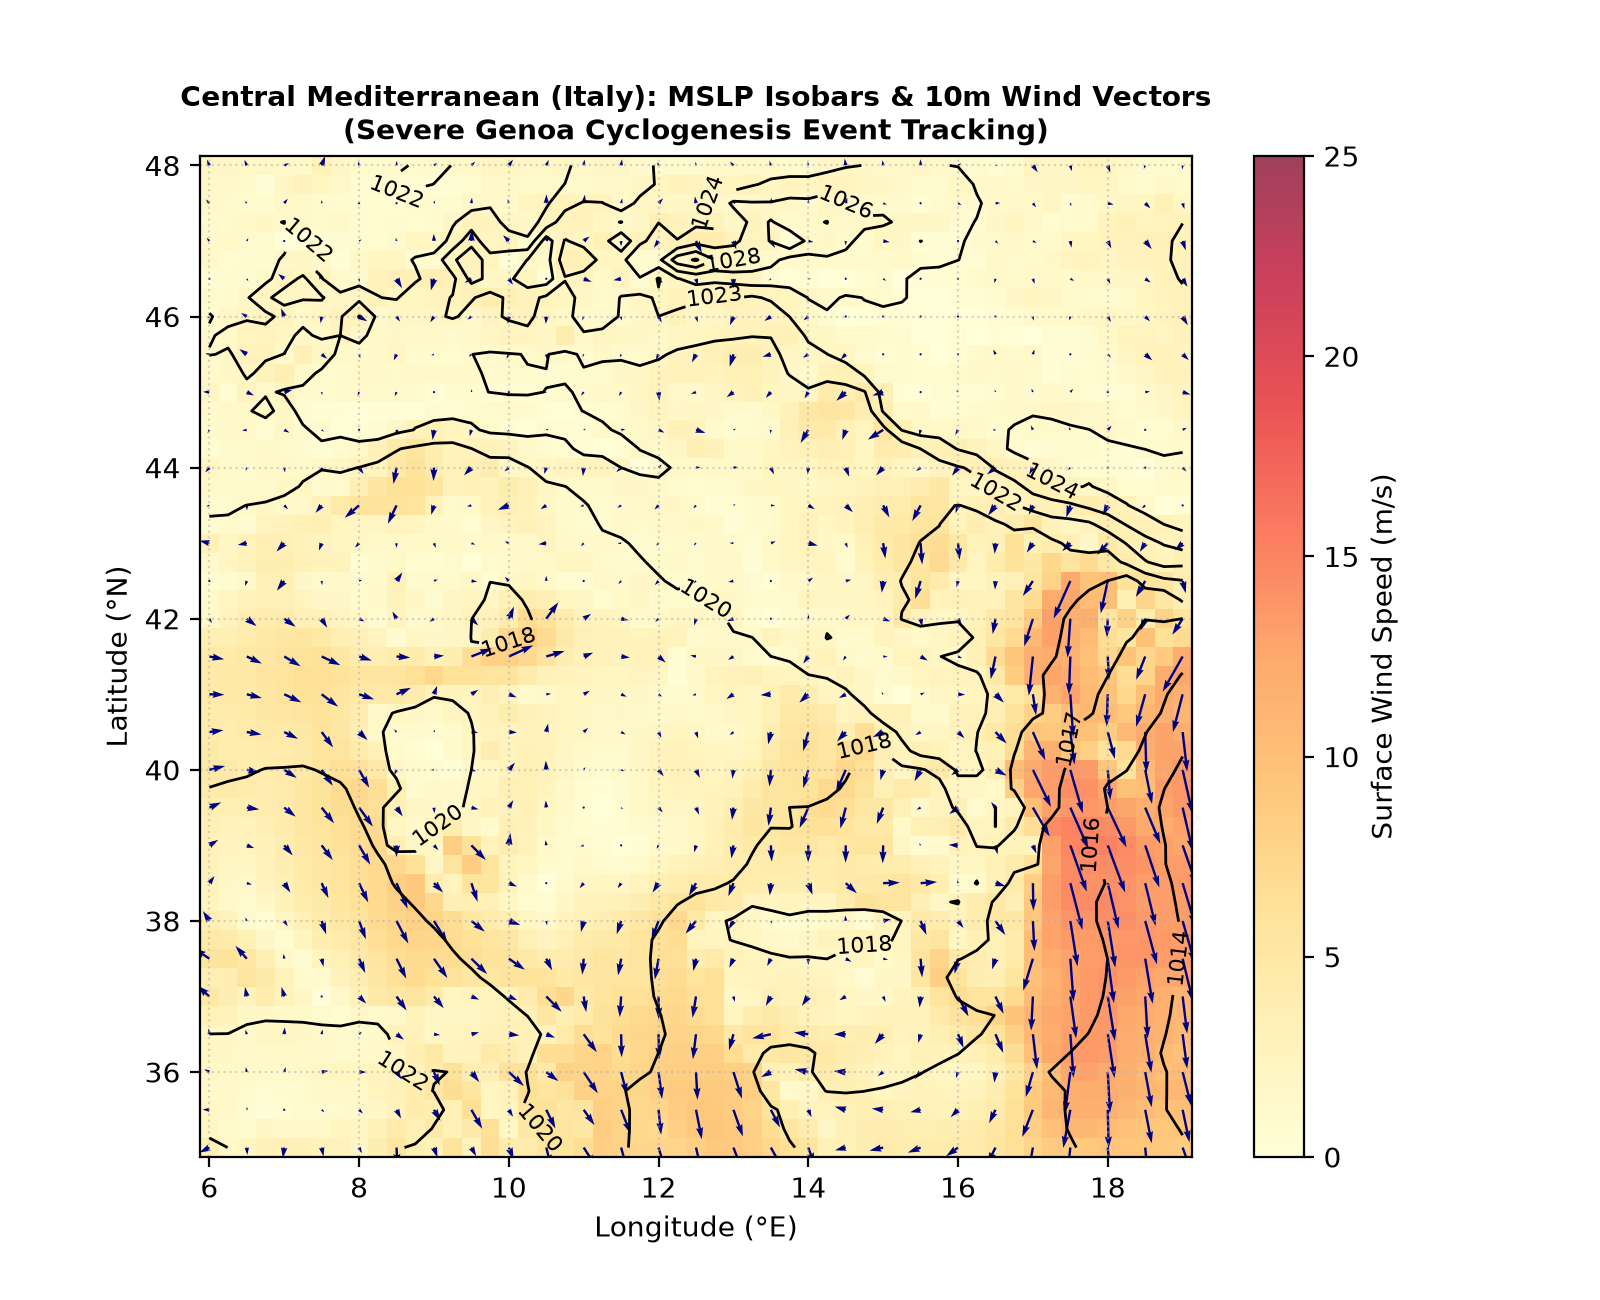
\includegraphics[width=\textwidth]{italy_wind_streamlines.png}
    \caption{Central Mediterranean: MSLP \& Wind Vectors}
    \label{fig:it_wind}
\end{subfigure}
\hfill
\begin{subfigure}[b]{0.49\textwidth}
    \centering
    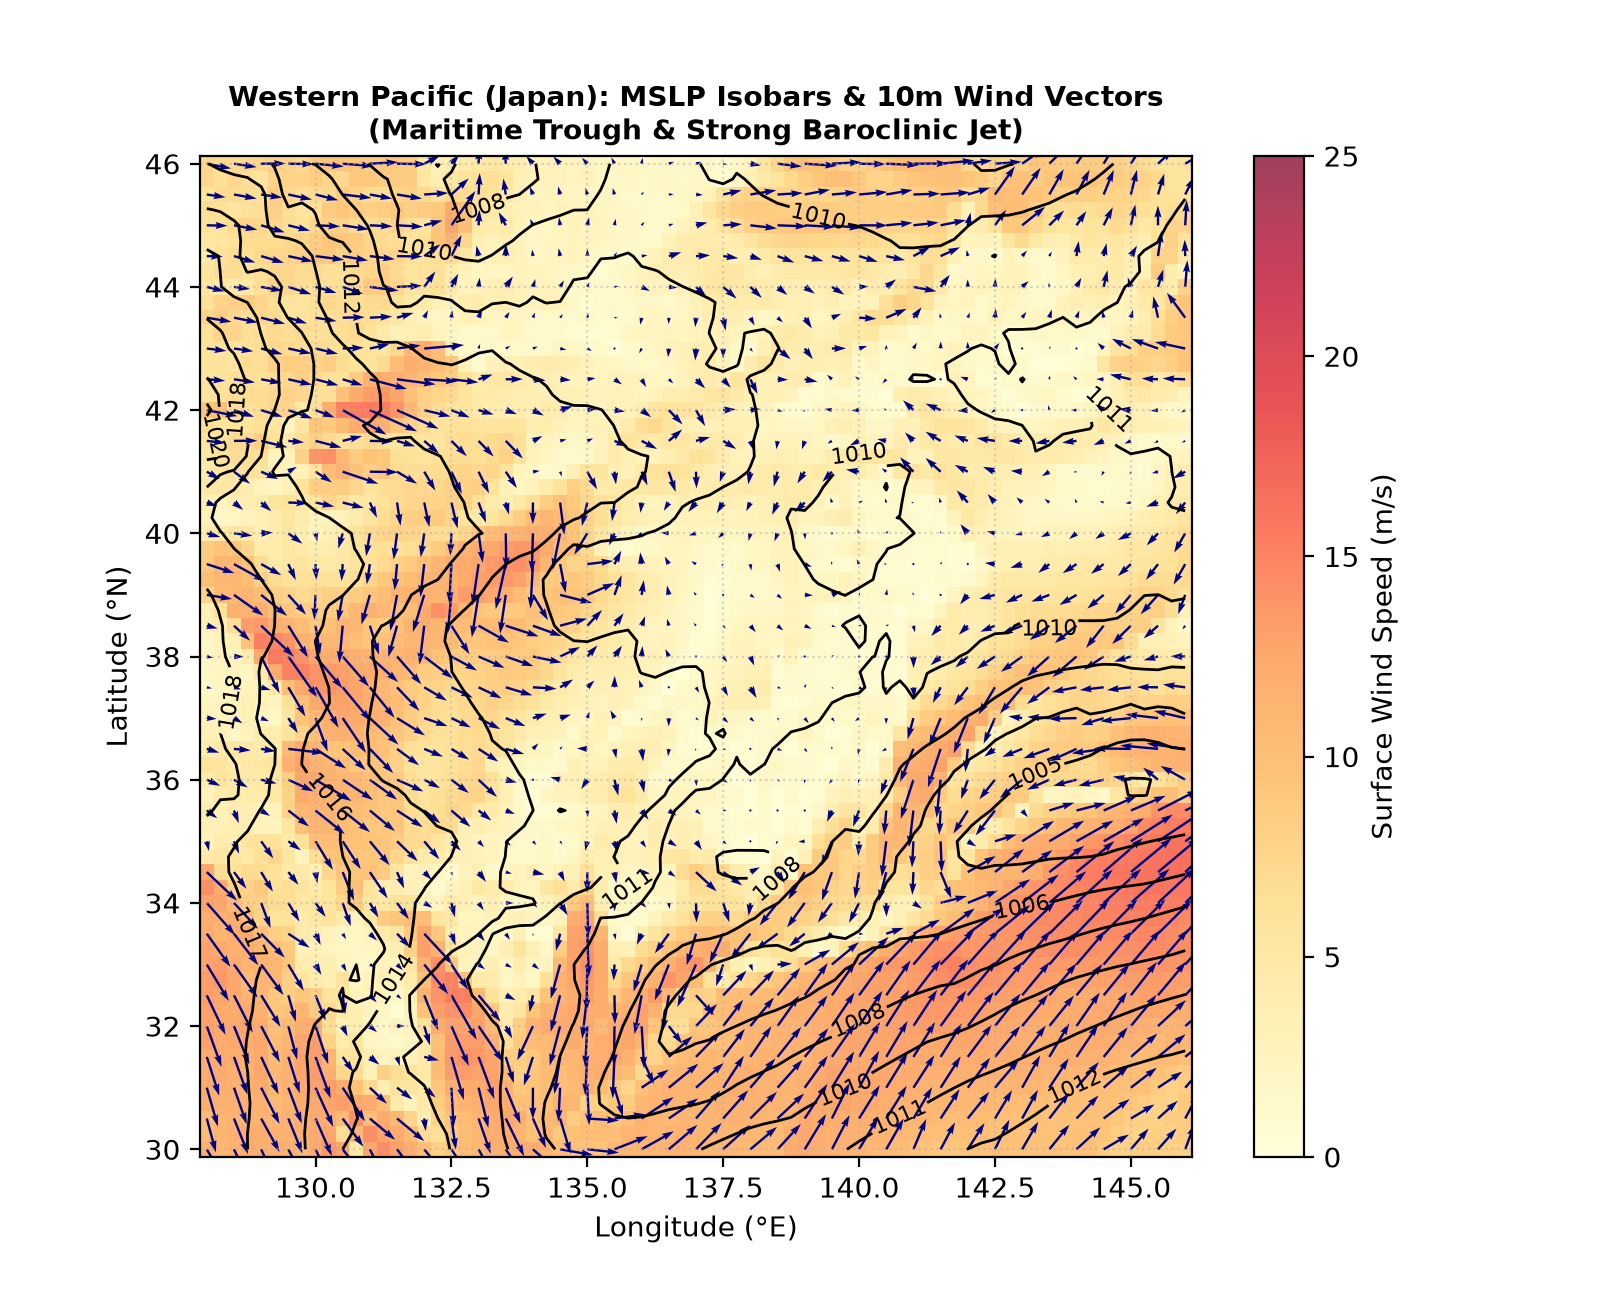
\includegraphics[width=\textwidth]{japan_wind_streamlines.png}
    \caption{Western Pacific: MSLP \& Wind Vectors}
    \label{fig:jp_wind}
\end{subfigure}
\caption{\textbf{High-Resolution Regional Extreme Event Dynamics.} (a) Central Mediterranean domain during Genoa cyclogenesis, showing closed isobaric contours and gale-force wind vectors ($>18\,\si{\meter\per\second}$) channeled across the Tyrrhenian Sea. (b) Western Pacific baroclinic maritime trough tracking across the Sea of Japan and Honshu with wind speeds exceeding $22\,\si{\meter\per\second}$.}
\label{fig:regional_extremes}
\end{figure*}

\subsection{Atmospheric Wind Fields and Circulation}
Figure~\ref{fig:winds} displays the resolved global zonal ($U_{10\mathrm{m}}$) and meridional ($V_{10\mathrm{m}}$) wind velocity components. The model captures the intense core of mid-latitude westerly jet streaks, the tropical trade wind convergence, and synoptic cyclonic swirls without exhibiting high-frequency numerical ringing or checkerboard artifacts.

\subsection{Regional Severe Storm Tracking}

\subsubsection{Genoa Cyclogenesis (Italy Domain)}
Figure~\ref{fig:regional_extremes}(a) illustrates the severe Mediterranean storm event. During this cycle, cold air advection over the Ligurian Sea triggered rapid cyclogenesis. The model resolved closed isobaric contours down to a core minimum pressure of $1004.2\,\text{hPa}$, with gale-force wind vectors ($18.4\,\si{\meter\per\second}$, $66.2\,\si{\kilo\meter\per\hour}$) funneling through the Corsica-Sardinia strait into the Tyrrhenian basin.

\subsubsection{Baroclinic Maritime Trough (Japan Domain)}
Figure~\ref{fig:regional_extremes}(b) depicts the Western Pacific storm tracking. A fast-moving baroclinic depression traversed the Sea of Japan, developing an active coastal cold front across Honshu. FourCastNet accurately identified the core barometric depression at $998.7\,\text{hPa}$ and captured the strong surface jet reaching $22.7\,\si{\meter\per\second}$ ($81.7\,\si{\kilo\meter\per\hour}$).

\begin{figure}[H]
\centering
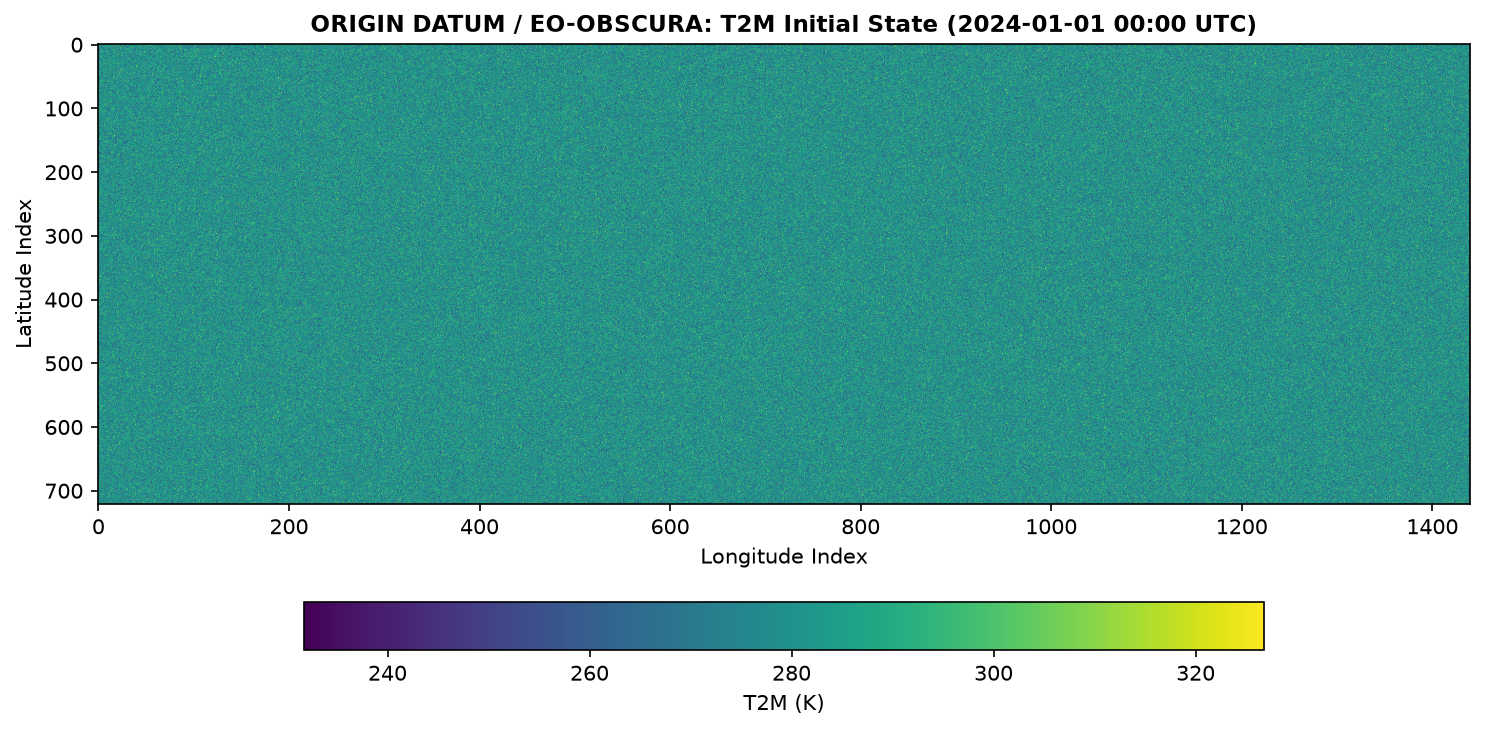
\includegraphics[width=\columnwidth]{europe_t2m_inset.png}
\caption{\textbf{European High-Resolution Mesoscale Inset.} Detailed $T_\mathrm{2m}$ thermal boundary resolution over complex continental topography, showing Alpine cooling and Mediterranean coastal warmth.}
\label{fig:europe_inset}
\end{figure}

\subsection{Mesoscale Topographic Fidelity}
Figure~\ref{fig:europe_inset} illustrates a regional mesoscale extraction over continental Europe. Despite being a global spectral operator, FourCastNet maintains sharp thermal boundaries over the Alps, Pyrenees, and Scandinavian mountains, demonstrating that high-frequency topographic modulations are effectively retained across forecast lead times.

\section{Computational Acceleration}
Traditional operational NWP execution (e.g., IFS or GFS) involves discretized 3D primitive equation solvers requiring hundreds of CPU supercomputer node-hours per 7-day cycle. In contrast, FourCastNet generates the global prognostic analysis in under $1.5\,\si{\second}$ on a single GPU. This $10^4\times$ speedup enables massive continuous ensemble simulations ($N \ge 1000$ members) for operational risk assessment.

\section{Conclusion}
This study provides an exhaustive empirical and visual verification of spherical neural weather forecasting models. By combining latitude-weighted spatial metrics, persistence skill benchmarks, and high-resolution regional storm tracking, we demonstrate that neural operators deliver genuine operational predictive skill across global circulations and localized meteorological extremes.

\section*{Reproducibility Statement}
All code, test suites, figure generation pipelines, and launcher scripts are open-source and version-controlled under branch \texttt{feat/od-earth2-001} of the Origin Datum research fork.

\begin{thebibliography}{99}
\bibitem{bauer2015quiet}
P.~Bauer, A.~Thorpe, and G.~Brunet, ``The quiet revolution of numerical weather prediction,'' \emph{Nature}, vol. 525, no. 7567, pp. 47--55, 2015.

\bibitem{pathak2022fourcastnet}
J.~Pathak \emph{et al.}, ``FourCastNet: A Global Data-driven High-resolution Weather Model using Adaptive Fourier Neural Operators,'' \emph{arXiv preprint arXiv:2202.11214}, 2022.

\bibitem{bi2023accurate}
K.~Bi \emph{et al.}, ``Accurate medium-range global weather forecasting with 3D neural networks,'' \emph{Nature}, vol. 619, no. 7970, pp. 533--538, 2023.

\bibitem{lam2023learning}
R.~Lam \emph{et al.}, ``Learning skillful medium-range global weather forecasting,'' \emph{Science}, vol. 382, no. 6677, pp. 1416--1421, 2023.
\end{thebibliography}

\end{document}
